\chapter{Algunas aplicaciones}

\lettrine [lines=5] {\initfamily \selectfont E} {ste} último capítulo está dedicado a la exploración de algunas de las diversas consecuencias que ha tenido la combinación del Algebra Lineal y la Teoría de Gráficas. Advertimos al lector que muchos de los teoremas que estableceremos aquí quedarán sin demostración pues están fuera del alcance de la tesis. 


\section{Otras matrices asociadas a gráficas y digráficas}
Al final del capítulo anterior hicimos uso de ciertas matrices con el propósito de construir bases para los espacios $\mathcal{B}(D)$ y $\mathcal{C}(D)$. En esta sección exploraremos con más detalle estás ideas \footnote{Puede consultarse \cite{Deo,Seshu,Gross}}. Como es costumbre, supondremos de ahora en adelante que $G$ es una gráfica, con $n$ vértices y $m$ aristas, con $k$ conjuntos de corte minimales: $B_{1}, \ldots, B_{k}$; y $q$ ciclos: $C_{1},\ldots, C_{q}$.

De igual manera, $D$ denotará una digráfica, con $n$ vértices y $m$ arcos. También supondremos que tiene $k$ cortes minimales y $q$ ciclos, para los cuales usaremos la misma notación que los cortes y ciclos de $G$.

$T$ denotará un árbol generador maximal tanto para $G$ como para $D$.

\subsection{Matriz de cortes}
Definimos la \textit{matriz de cortes de $G$} como aquella matriz $\mathbf{B} \in \mathbb{M}_{k \times m}(GF(2))$ cuyos renglones son:
$$
\mathbf{B}:= \begin{bmatrix} 
\boldsymbol{\chi}_{B_{1}}^{\mathbf{t}} \\
\-- \\
\vdots
\-- \\
\boldsymbol{\chi}_{B_{k}}^{\mathbf{t}}
\end{bmatrix}.
$$
 Es decir, los renglones de $\mathbf{B}$ son los vectores de incidencia de los conjuntos de corte minimales de $G$. En el inciso (a) de la figura \ref{fig:matrizdecortes} se encuentran una gráfica y su matriz $\mathbf{B}$.
 
 Por el desarrollo hecho en el capítulo anterior, es sencillo darse cuenta que $\mathsf{R}(\mathbf{B}) =\overrightarrow{\mathcal{B}}(G)$ y, por tanto, $Ker(\mathbf{B}) = \overrightarrow{\mathcal{C}}(G)$. Luego, $rank(\mathbf{B}) = \rho(G)$ y $null(\mathbf{B}) = \mu(G)$.
 
Si $H$ es una subgráfica generadora de $G$, su respectiva matriz de cortes $\mathbf{B}_{H}$ está conformada por los renglones de la forma $\boldsymbol{\chi}_{B_{i} \cap H}^{\mathbf{t}}$, $i\in\{1, \ldots, k\}$ (ya que $H$ conserva los mismos vértices de $G$). 

Hay un resultado análogo al teorema \ref{teo:liaciclicas} (cuya demostración también similar):
\begin{teo}\label{teo:limatrizcortes}
Si $S\subseteq E(G)$ entonces el conjunto de columnas de $\mathbf{B}$ asociadas a $S$, $\{\mathbf{b}_{a}| a \in S\}$, es linealmente independiente si y sólo si $G[S]$ es acíclica.
\end{teo}

\begin{cor} Sea
$S \subseteq E(G)$. Entonces $\{\mathbf{b}_{e} | e \in S\}$ es una base para el espacio de columnas $\mathsf{C}(\mathbf{B})$ si y sólo si $G[S]$ es un bosque generador maximal. Por lo tanto, las bases de $\mathsf{C}(\mathbf{B})$ están en corespondencia uno a uno con los bosques generadores maximales de $G$.
\end{cor} 

Hasta aquí, el lector podrá darse cuenta que las matrices de corte y las de incidencias son muy parecidas.

Una \textit{matriz base de cortes} es una matriz cuyos renglones forman una base para el espacio $\overrightarrow{\mathcal{B}}(D)$. Obsérvese que su tamaño es $\rho(G) \times m$. Es sencillo verificar que estas matrices cumplen el teorema anterior. Aún más, podemos confirmar lo siguiente.

\begin{teo} \label{teo:submatricesmatridecortes}
Si $\mathbf{Q}$ es una matriz base de cortes, entonces cualquiera de sus submatrices cuadradas, de tamaño $\rho \times \rho$, es no singular si y sólo si sus columnas corresponden a las aristas de algún bosque generador maximal de $G$.
\end{teo}

Una matriz base de cortes, en particular, es la matriz $\mathbf{B}_{f}$ en la que sus renglones corresponden a cortes fundamentales respecto a algún bosque generador maximal. En el inciso $(b)$ de la figura \ref{fig:matrizdecortes} mostramos la matriz $\mathbf{B}_{f}$ respecto al árbol generador cuyas ramas se han resaltado.

\begin{figure}[h]
    \centering
    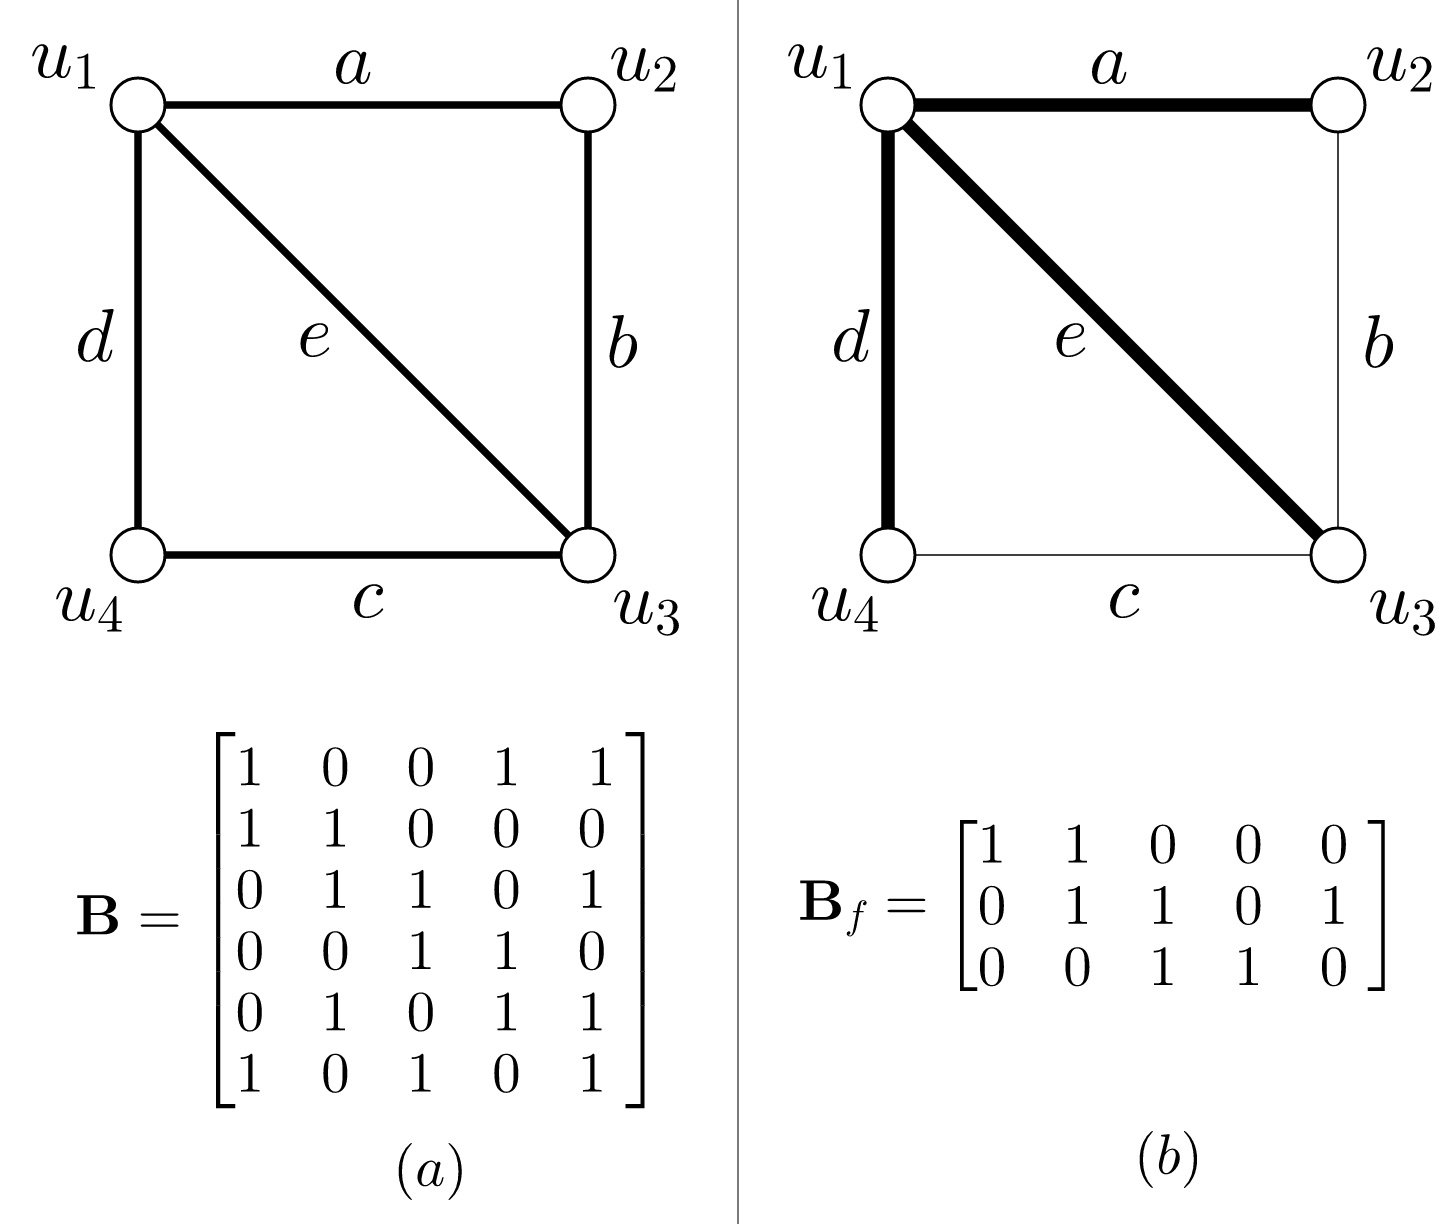
\includegraphics[scale=0.25]{img/imgchapter4/matrizdecortes.jpg}
    \caption{}
    \label{fig:matrizdecortes}
\end{figure}

Tomemos $T$ un bosque generador maximal de $G$. Notemos que si ordenamos las aristas de $G$ como $E(G) = E(\overline{T}) \cup E(T)$ y a los cortes fundamentales de tal forma que sus ramas coincidan con el orden de $E(T)$, entonces podemos reescribir a la matriz $\mathbf{B}_{f}$ como
$$
\mathbf{B}_{f} = \begin{bmatrix}
\mathbf{\overline{T}} & | & \mathbf{I}_{\rho}
\end{bmatrix}.
$$

En cuanto a las digráficas, los conceptos son análogos. La \textit{matriz de cortes de la digráfica de $D$} es la matriz $\mathbf{B} \in \mathbb{M}_{k\times m}(\mathbb{R})$ cuyos renglones son las tensiones asociadas a sus cortes minimales, i.e., $$ 
\mathbf{B}:= \begin{bmatrix} 
\mathbf{g}_{B_{1}}^{\mathbf{t}} \\
\-- \\
\vdots
\-- \\
\mathbf{g}_{B_{k}}^{\mathbf{t}}
\end{bmatrix}.
$$

Es fácil deducir que  $\mathsf{R}(\mathbf{B}) =\mathcal{B}(D)$ y, por tanto, $Ker(\mathbf{B}) = \mathcal{C}(D)$. Luego, $rank(\mathbf{B}) = \rho(D)$ y $null(\mathbf{B}) = \mu(D)$. Véase la figura \ref{fig:matrizdecortesdirigidos}.

Una \textit{matriz base de cortes de $D$} es la matriz cuyos renglones son una base para el espacio de tensiones $\mathcal{B}(D)$. Además las relaciones de dependencia lineal que se tenían para gráficas, aquí también se siguien cumpliendo, esto es, que las columnas linealmente independientes de $\mathbf{B}$ corresponden a digráficas sin ciclos.

$\mathbf{B}_{f}$ también denota a la matriz base de cortes cuyos renglones son las tensiones fundamentales asociadas a un árbol generador maximal de $D$. Por supuesto, ordenando de manera adecuada las tensiones fundamentales y los arcos $A(D) = A(\overline{T}) \cup A(T)$, podemos escribir:
$$
\mathbf{B}_{f} = \begin{bmatrix}
\mathbf{\overline{T}}& | & \mathbf{I}_{\rho}
\end{bmatrix}.
$$

\begin{figure}[h]
    \centering
    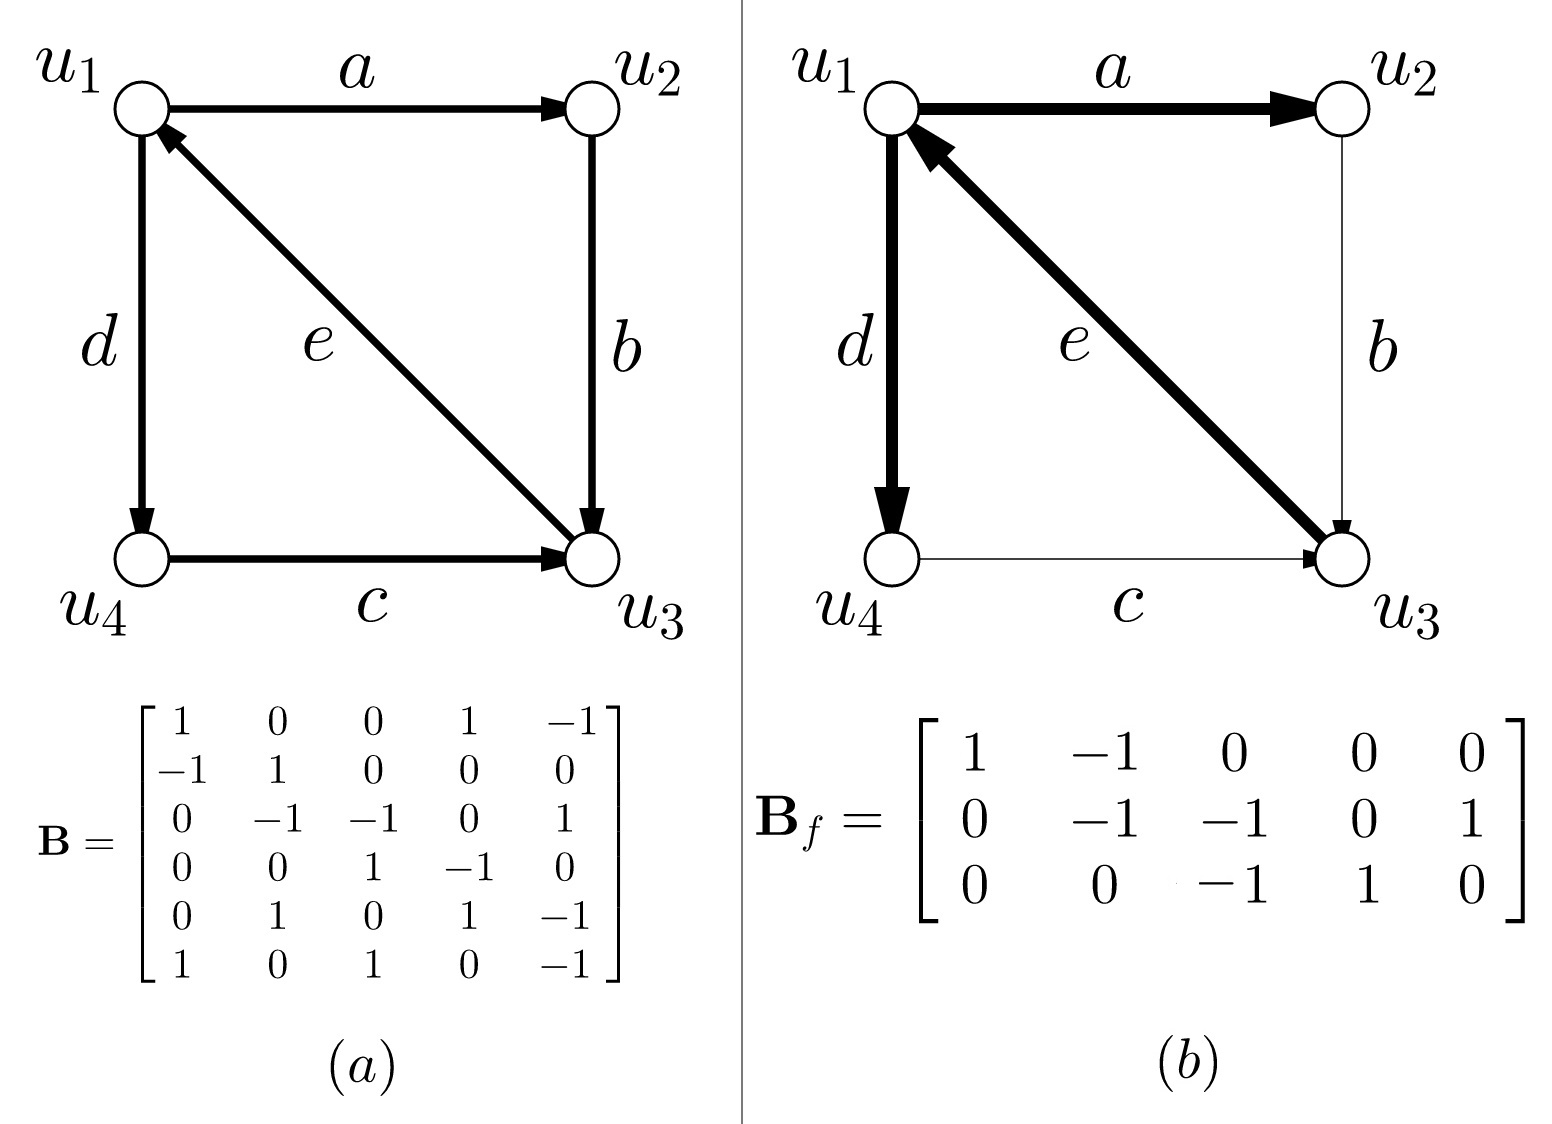
\includegraphics[scale=0.25]{img/imgchapter4/matrizdecortesdirigidos.jpg}
    \caption{}
    \label{fig:matrizdecortesdirigidos}
\end{figure}

\subsection{Matriz de ciclos}

La \textit{matriz de ciclos de $G$} es la matriz $\mathbf{C} \in \mathbb{M}_{q \times m}(\mathbb{R})$ de la forma: $$\mathbf{C}:= \begin{bmatrix} 
\boldsymbol{\chi}_{C_{1}}^{\mathbf{t}} \\
\-- \\
\vdots
\-- \\
\boldsymbol{\chi}_{C_{q}}^{\mathbf{t}}
\end{bmatrix},
$$ 
donde cada $\boldsymbol{\chi}_{C_{i}}^{\mathbf{t}}$ es el vector de incidencia del ciclo $C_{i}$, $i \in \{1,\ldots, q\}$. En la imagen \ref{fig:matrizdeciclos} mostramos la matriz $\mathbf{C}$ de la figura \ref{fig:matrizdecortes}.

 Debido a la definición de esta matriz, podemos darnos cuenta que $\mathsf{R}(\mathbf{C}) =\overrightarrow{\mathcal{C}}(G)$ y, por tanto, $Ker(\mathbf{C}) = \overrightarrow{\mathcal{B}}(G)$. Luego, $rank(\mathbf{C}) = \mu(G)$ y $null(\mathbf{C}) = \rho(G)$.
 
 Lo anterior implica un teorema \textit{dual} al \ref{teo:limatrizcortes}:
 
\begin{teo}\label{teo:limatrizciclos}
Si $S\subseteq E(G)$ entonces el conjunto de columnas de $\mathbf{C}$ asociadas a $S$, $\{\mathbf{c}_{a}| a \in S\}$, es linealmente independiente si y sólo si $G[S]$ no contiene cortes minimales.
\end{teo}

 
 Entonces \textit{$G[S]$ contiene un corte minimal si y sólo si $\{\mathbf{c}_{a} | a \in S\}$ es un conjunto linealmente dependiente}. Además, los conjuntos de aristas más grandes posibles, que no desconectan una gráfica, son los complementos de los árboles generadores maximales, como lo afirmamos en el siguiente corolario.

\begin{cor} Sea
$S \subseteq E(G)$. Entonces $\{\mathbf{c}_{e} | e \in S\}$ es una base para el espacio de columnas $\mathsf{C}(\mathbf{C})$ si y sólo si $G[S]$ es el complemento de un bosque generador maximal. Por lo tanto, las bases de $\mathsf{C}(\mathbf{C})$ están en corespondencia uno a uno con los complementos de bosques generadores maximales de $G$.
\end{cor} 

\begin{figure}[h]
    \centering
    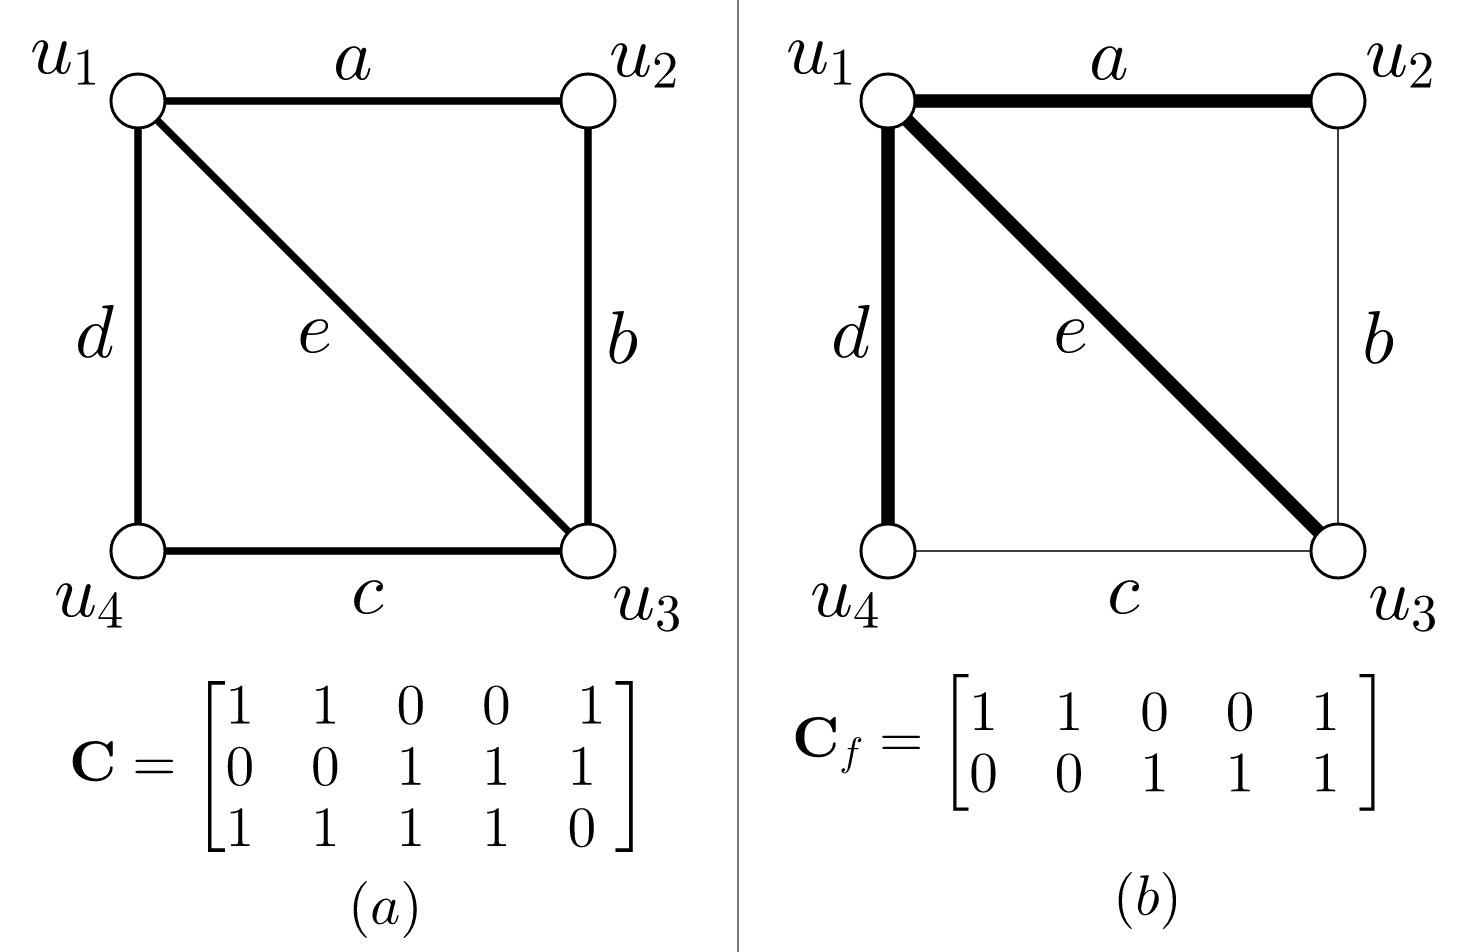
\includegraphics[scale=0.25]{img/imgchapter4/matrizdeciclos.jpg}
    \caption{}
    \label{fig:matrizdeciclos}
\end{figure}

Una \textit{matriz base de ciclos} es una matriz cuyos renglones forman una base para el espacio $\overrightarrow{\mathcal{C}}(D)$. Obsérvese que su tamaño es $\mu(G) \times m$. Además de que estás matrices cumplen las proposiciones previas, también tenemos lo siguiente.

\begin{teo} \label{teo:submatricesmatridecortes}
Si $\mathbf{Q}$ es una matriz base de ciclos, entonces cualquiera de sus submatrices cuadradas, de tamaño $\mu \times \rho$, es no singular si y sólo si sus columnas corresponden a las cuerdas del complemento de algún bosque generador maximal de $G$.
\end{teo}

Una matriz base de ciclos es la matriz $\mathbf{C}_{f}$ en las que sus renglones corresponden a los ciclos fundamentales respecto a algún bosque generador maximal. En el inciso $(b)$ de la figura \ref{fig:matrizdeciclos} mostramos la matriz $\mathbf{C}_{f}$ respecto al árbol generador de la figura \ref{fig:matrizdecortes}.

Tomemos $T$ un bosque generador maximal de $G$. Ordenando las aristas de $G$ como $E(G) = E(\overline{T}) \cup E(T)$ y a sus ciclos fundamentales de tal forma que sus cuerdas coincidan con el orden de $E(\overline{T})$, podemos reescribir a la matriz $\mathbf{C}_{f}$ como
$$
\mathbf{C}_{f} = \begin{bmatrix}
\mathbf{I}_{\mu} & | & \mathbf{T}
\end{bmatrix}.
$$

Respecto a las digráficas, las definiciones son parecidas. La \textit{matriz de ciclos de la digráfica de $D$} es la matriz $\mathbf{C} \in \mathbb{M}_{q\times m}(\mathbb{R})$ cuyos renglones son las circulaciones asociadas a sus ciclos, i.e., $$ 
\mathbf{C}:= \begin{bmatrix} 
\mathbf{f}_{C_{1}}^{\mathbf{t}} \\
\-- \\
\vdots
\-- \\
\mathbf{f}_{C_{k}}^{\mathbf{t}}
\end{bmatrix}.
$$

Notemos que  $\mathsf{R}(\mathbf{C}) =\mathcal{C}(D)$ y, por tanto, $Ker(\mathbf{C}) = \mathcal{B}(D)$. Luego, $rank(\mathbf{C}) = \mu(D)$ y $null(\mathbf{C}) = \rho(D)$. Véase la figura \ref{fig:matrizdeciclosdirigidos}.

Una \textit{matriz base de ciclos de $D$} es la matriz cuyos renglones son una base para el espacio de circulaciones $\mathcal{C}(D)$. Además las relaciones de dependencia lineal que se tenían para gráficas, aquí también se siguien cumpliendo, esto es, que las columnas linealmente independientes de $\mathbf{C}$ corresponden a digráficas que no contienen cortes minimales.

$\mathbf{C}_{f}$ también denota a la matriz base de cortes cuyos renglones son las circulaciones fundamentales asociadas a un árbol generador maximal de $D$. Ordenando de manera adecuada las circulaciones fundamentales y los arcos $A(D) = A(\overline{T}) \cup A(T)$, podemos escribir:
$$
\mathbf{C}_{f} = \begin{bmatrix}
\mathbf{I}_{\mu} & | & \mathbf{T}
\end{bmatrix}.
$$
\begin{figure}[h]
    \centering
    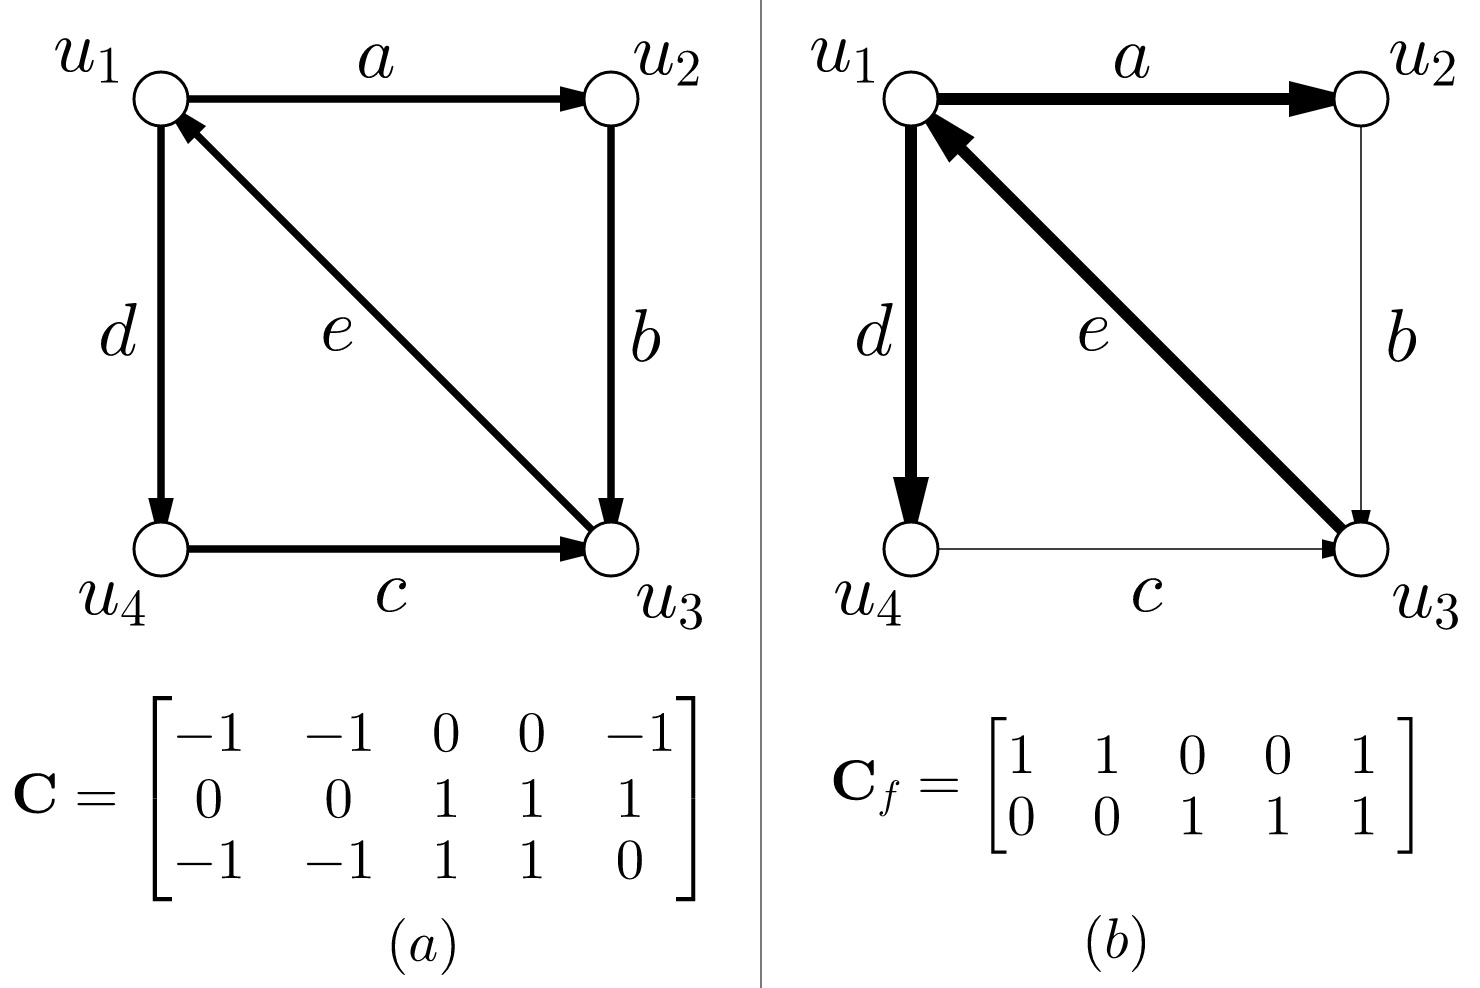
\includegraphics[scale=0.25]{img/imgchapter4/matrizdeciclosdirigidos.jpg}
    \caption{}
    \label{fig:matrizdeciclosdirigidos}
\end{figure}

\subsection{Relaciones entre las matrices $\mathbf{M}$, $\mathbf{B}$ y $\mathbf{C}$}

Ya sean gráficas dirigidas o no, vimos en el capítulo anterior que los ciclos y los cortes son ortogonales, así como las circulaciones y las tensiones. Debido a sus definiciones, la propiedad de ortogonalidad repercute en las matrices que hemos estudiado en estas secciones.

\begin{teo}
Supongamos que $\mathbf{M}$, $\mathbf{B}$ y $\mathbf{C}$ son las matrices de incidencia, de cortes y de ciclos (de tensiones y de circulaciones), respectivamente, de una gráfica (de una digráfica). Si asumimos que tales matrices tiene el mismo orden de columnas, entonces se cumplen las siguientes igualdades: $\mathbf{M}\mathbf{C^{t}} = \mathbf{O}$, $\mathbf{C}\mathbf{M^{t}} = \mathbf{O}$, $\mathbf{B}\mathbf{C^{t}} = \mathbf{O}$ y $\mathbf{C}\mathbf{B^{t}} = \mathbf{O}$.

Aún más, si $\mathbf{\widehat{M}}$ es la matriz de incidencia reducida, y $\mathbf{B}_{f}$ y $ \mathbf{C}_{f}$ son las matrices base de cortes y ciclos (tensiones y circulacones) fundamentales respecto a un bosque generador maximal, también se cumple que: $\mathbf{\widehat{M}}\mathbf{C}_{f}^{\mathbf{t}} = \mathbf{O}$, $\mathbf{C}_{f}\mathbf{\widehat{M}^{t}} = \mathbf{O}$, $\mathbf{B}_{f}\mathbf{C}_{f}^{\mathbf{t}} = \mathbf{O}$ y $\mathbf{C}_{f}\mathbf{B}_{f}^{\mathbf{t}}= \mathbf{O}$.
\end{teo}

Recordando que las submatrices cuadradas de $n-c \times n-c$, no singulares, de $\mathbf{\widehat{M}}$ corresponden bosques generadores maximales, enunciamos el corolario que sigue.

\begin{cor}
Sea $T$ un bosque generador maximal de una gráfica $G$ (o de una digráfica $D$). Supongamos que las columnas de las matrices  $\mathbf{\widehat{M}}$, $\mathbf{B}_{f}$, $\mathbf{C}_{f}$ se han arreglado según $E(G) = E(\overline{T}) \cup E(T)$ (o $A(D) = A(\overline{T}) \cup A(T)$), de forma que $\mathbf{\widehat{M}} = \begin{bmatrix} \mathbf{\widehat{M}}_{\overline{T}} & |& \mathbf{\widehat{M}}_{T} \end{bmatrix}$, $\mathbf{B}_{f} = \begin{bmatrix} \mathbf{\overline{T}} & |& \mathbf{I}_{\rho} \end{bmatrix}$ y $\mathbf{C}_{f} = \begin{bmatrix} \mathbf{I}_{\mu} & |& \mathbf{T} \end{bmatrix}$. Entonces podemos afirmar que las matrices de cortes y ciclos fundamentales (tensiones y circulaciones)son de la forma:
\begin{align*}
    \mathbf{B}_{f} &= \begin{bmatrix} \mathbf{\widehat{M}}_{T}^{-1}\mathbf{\widehat{M}}_{\overline{T}} & |& \mathbf{I}_{\rho} \end{bmatrix} \\
    \mathbf{C}_{f} &= \begin{bmatrix} \mathbf{I}_{\mu} & |& -\mathbf{\widehat{M}}_{\overline{T}}^{\mathbf{t}}(\mathbf{\widehat{M}}_{T}^{\mathbf{t}})^{-1}  \end{bmatrix}
\end{align*}
\end{cor}

Lo anterior significa que, a partir de la matriz de incidencia y un bosque generador maximal, podemos construir los cortes (tensiones) y ciclos (circulaciones) fundamentales de una gráfica (digráfica).

\section{¿Cuántos árboles generadores tiene una gráfica?}

$t(G)$ denota a la cantidad total de árboles generadores de una gráfica $G$ conexa. Se sabe que Arthur Cayley (1821 - 1895) estableció que hay $t(K_{n}) = n^{n-2}$ árboles generadores en una gráfica completa de $n$ vértices.

Las herramientas que hemos desarrollado en todo este trabajo nos permiten elaborar una fórmula que nos dice cuántos árboles generadores tiene una gráfica conexa arbitraria. 

Para lograr nuestro objetivo, haremos uso de la matriz de incidencia de una digráfica. Esta matriz es \textit{totalmente unimodular}, lo cual significa que cualquiera de sus submatrices cuadradas tiene determinante $1, -1$ ó $0$.

\begin{teo} \label{teo:totalmenteunimodular}
Dada $D$ una digráfica conexa, su matriz de incidencia $\mathbf{M}_{D}$ es totalmente unimodular.
\end{teo}

\begin{proof} Esta prueba se hace por inducción sobre el tamaño de las submatrices cuadradas. Téngase en cuenta que $\mathbf{M}$ es una matriz cuyas entradas son sólo $1, -1$ ó $0$. Así, una submatriz cuadrada de $1 \times 1$ tiene como única entrada alguno de esos valores, cumpliéndose el enunciado.

Supongamos que toda submatriz cuadrada de tamaño $(k-1) \times (k-1)$ de $\mathbf{M}$ tiene determinante $1, -1$ ó $0$. 

Sea $\textbf{A}$ una submatriz cuadrada de tamaño $k \times k$. Si $\textbf{A}$ tiene un renglón o una columna cuyas entradas son todas $0$, entonces $det(\textbf{A}) = 0$. Si todas las columnas de $\textbf{A}$ tiene exactamente un $1$ y un $-1$ en sus entradas, también $det(\textbf{A}) = 0$ pues si sumamos todos renglones de $\textbf{A}$, mediante operaciones elementales, obtendremos un renglón con todas sus entradas iguales a $0$, regresando al caso anterior.

El único caso restante es cuando $\textbf{A}$ tiene alguna columna con una única entrada con valor $1$ ó $-1$ (y las demás $0$). Utilizando la fórmula de Laplace y expandiendo el determinante sobre esta columna obtenemos que $$\textbf{A} = \pm 1 \cdot\widetilde{\textbf{A}}_{ij},$$ donde $\widetilde{\textbf{A}}_{ij}$ es una matriz de tamaño $(k-1) \times (k-1)$. De aquí que, por hipótesis de inducción, $det(\textbf{A}) \in \{-1, 0,1\}$. Por lo tanto, $\mathbf{M}$ es totalmente unimodular.

\end{proof}

\begin{cor}
La matriz de incidencia reducida de cualquier digráfica es totalmente unimodular.
\end{cor}

Haremos uso de una fórmula que nos permite calcular el determinante de un producto de matrices. La enunciaremos pero sin demostración \footnote{Puede hallarse una prueba en \cite{Deo}}. Antes debemos explicar nuestra notación: tomemos una matriz $\textbf{A}$, cuyo conjunto de columnas está indexado por un conjunto $E$. Si $S\subseteq E$, $\textbf{A}|_{S}$ es la submatriz de $\textbf{A}$ donde sus columnas son aquellas que corresponden a los elementos de $S$.

\begin{teo}[\textit{\textbf{Fórmula de Cauchy-Binet}}]

Sean $\mathbf{A}, \mathbf{B} \in \mathbb{M}_{k \times m}(\mathbb{R})$. Entonces 
$$
det(\mathbf{A}\mathbf{B^{t}}) = 
\sum_\big{S \in \binom{\{1,\ldots, m\}}{k}} det(\mathbf{A}|_{S}) \cdot det(\mathbf{B}|_{S}).
$$
\end{teo}

Ya tenemos  todo lo necesario para poder expresar el número de árboles generadores de una gráfica. Considerémos de antemano que los árboles generadores de una digráfica son los mismos de los de su gráfica subyacente (sin las orientaciones de las aristas). 

\begin{teo}[\textit{\textbf{El teorema Matriz-Árbol}}]
Sea $G$ una gráfica conexa, con $n$ vértices y $m$ aristas. De igual manera, sea $\overrightarrow{G}$ una orientación cualquiera de $G$. Entonces
$$
t(G) = det(\widehat{\mathbf{M}}_{\overrightarrow{G}}(\widehat{\mathbf{M}}_{\overrightarrow{G}})^{\mathbf{t}}).
$$
\end{teo}

\begin{proof}
Ya sabemos que las submatrices de $\widehat{\mathbf{M}}_{\overrightarrow{G}}$  de tamaño $(n-1) \times (n-1)$ son no singulares si las $n-1$ columnas corresponden a las aristas de un árbol generador de $G$; y estas submatrices tienen determinante $1$ ó $-1$ por el teorema \ref{teo:totalmenteunimodular}.

Por la fórmula de Cauchy-Binet y porque $\widehat{\mathbf{M}}_{\overrightarrow{G}}$ es totalmente unimodular, tenemos:
\begin{align*}
    det(\widehat{\mathbf{M}}_{\overrightarrow{G}}(\widehat{\mathbf{M}}_{\overrightarrow{G}})^{\mathbf{t}}) &= \sum_\big{S \in \binom{\{1,\ldots, m\}}{n-1}} det(\widehat{\mathbf{M}}_{\overrightarrow{G}}|_{S}) \cdot det(\widehat{\mathbf{M}}_{\overrightarrow{G}}|_{S})\\ &= \sum_\big{S \in \binom{\{1,\ldots, m\}}{n-1}} (det(\widehat{\mathbf{M}}_{\overrightarrow{G}[S]}))^{2} \\ &= \sum_\big{S \in \binom{\{1,\ldots, m\}}{n-1} \vspace{1em}}\{ 1 | \overrightarrow{G}[S] \textnormal{ es árbol generador} \} \\ &= t(G)
\end{align*}

\end{proof}

\begin{ejem}
Consideraremos la \textit{gráfica de Petersen} y su matriz de incidencia reducida, que se encuentran en la figura \ref{fig:petersen}.

\begin{figure}[H]
    \centering
    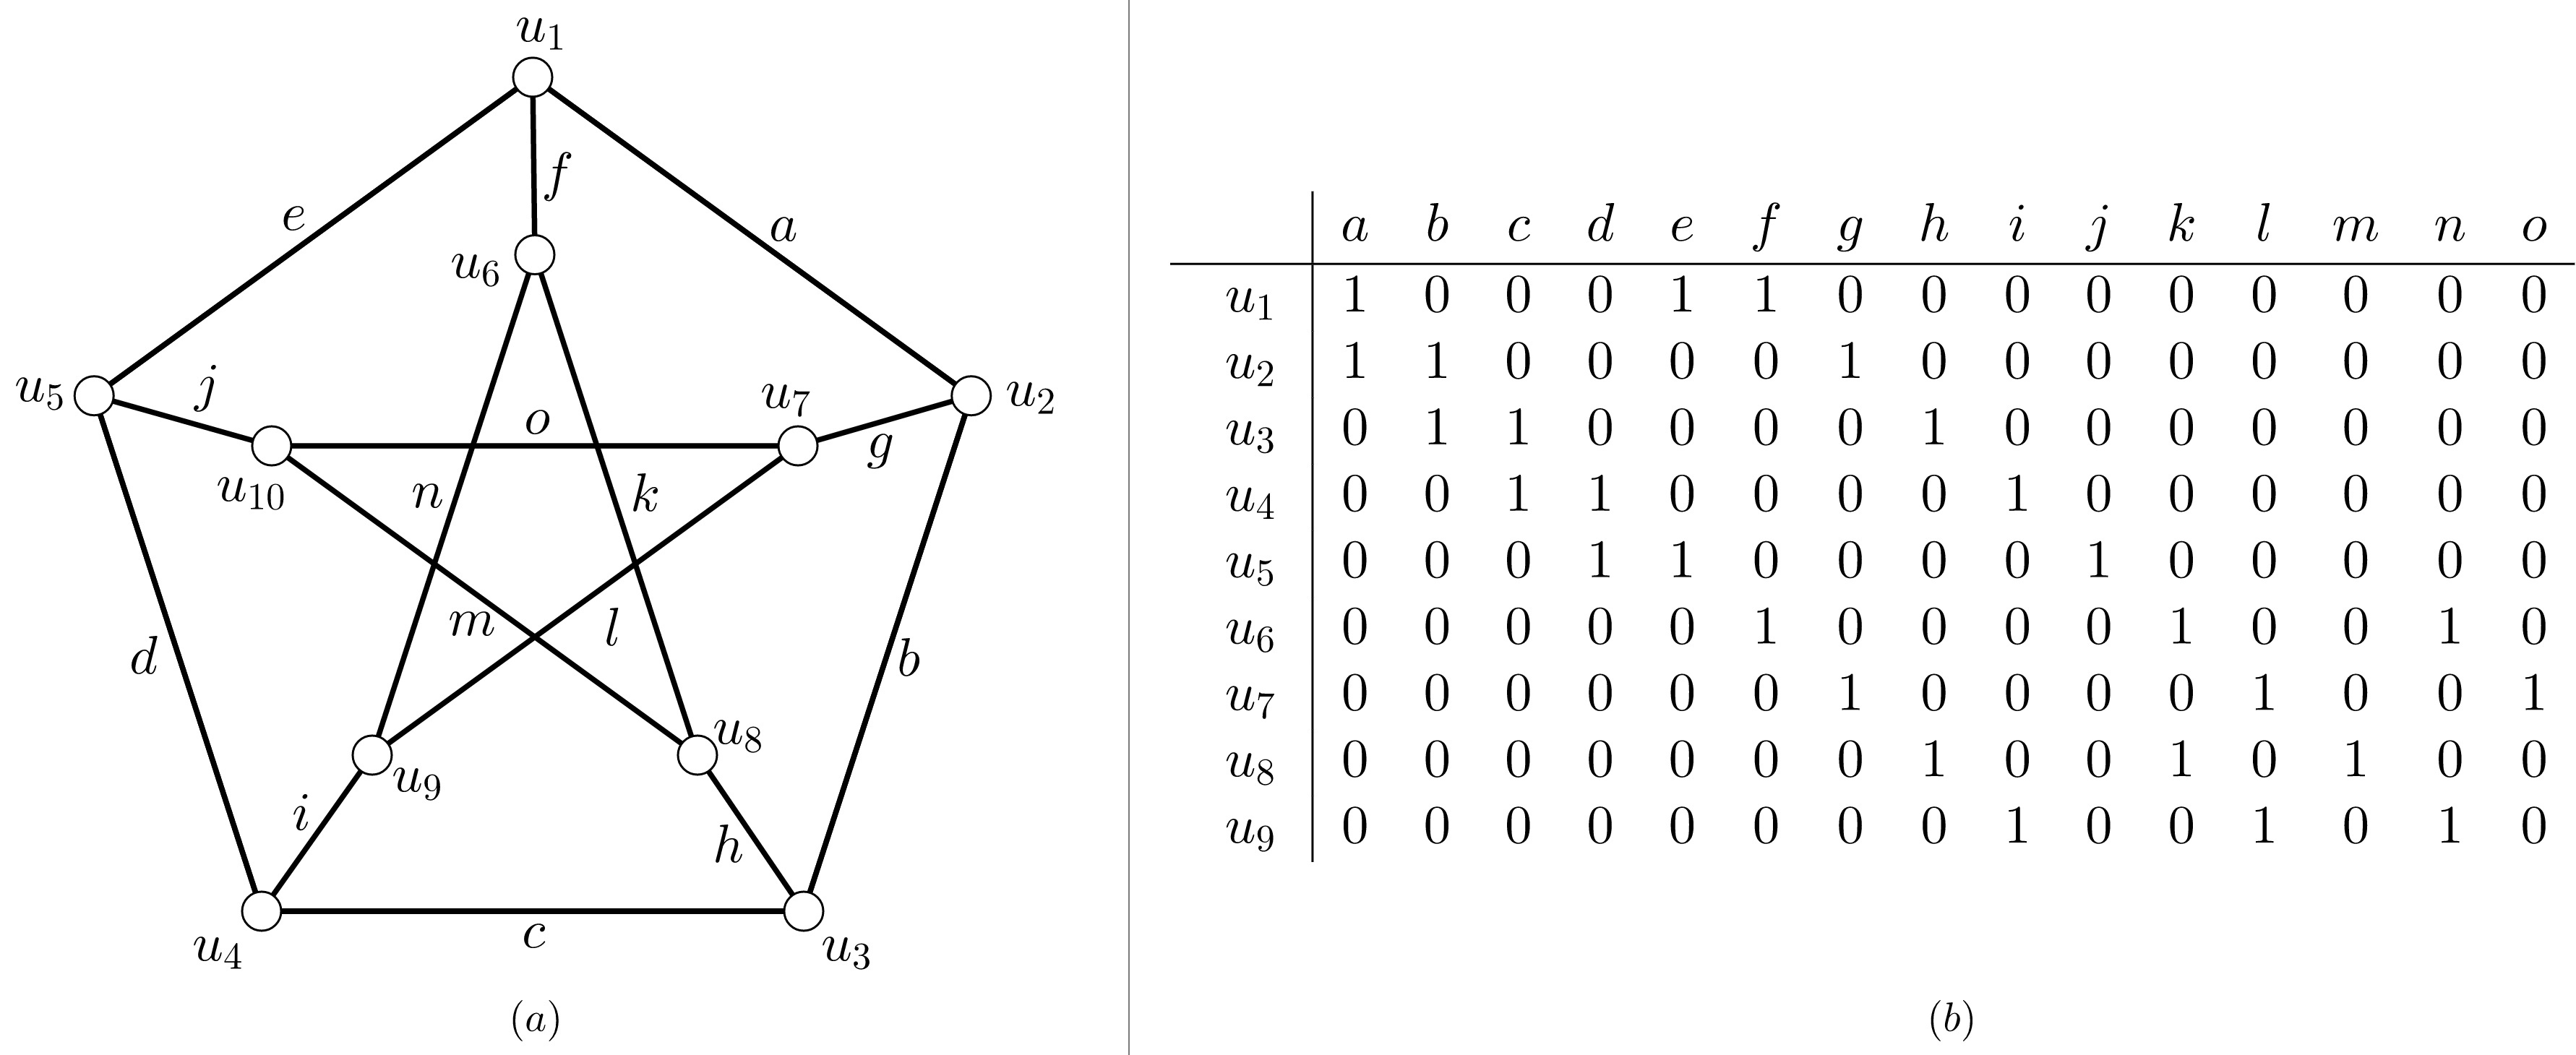
\includegraphics[scale=0.14]{img/imgchapter4/petersen.jpg}
    \caption{}
    \label{fig:petersen}
\end{figure}

Darle una orientación a esta gráfica se traduce en cambiar algún $1$ por un $-1$ en cada columna:

\begin{figure}[H]
    \centering
    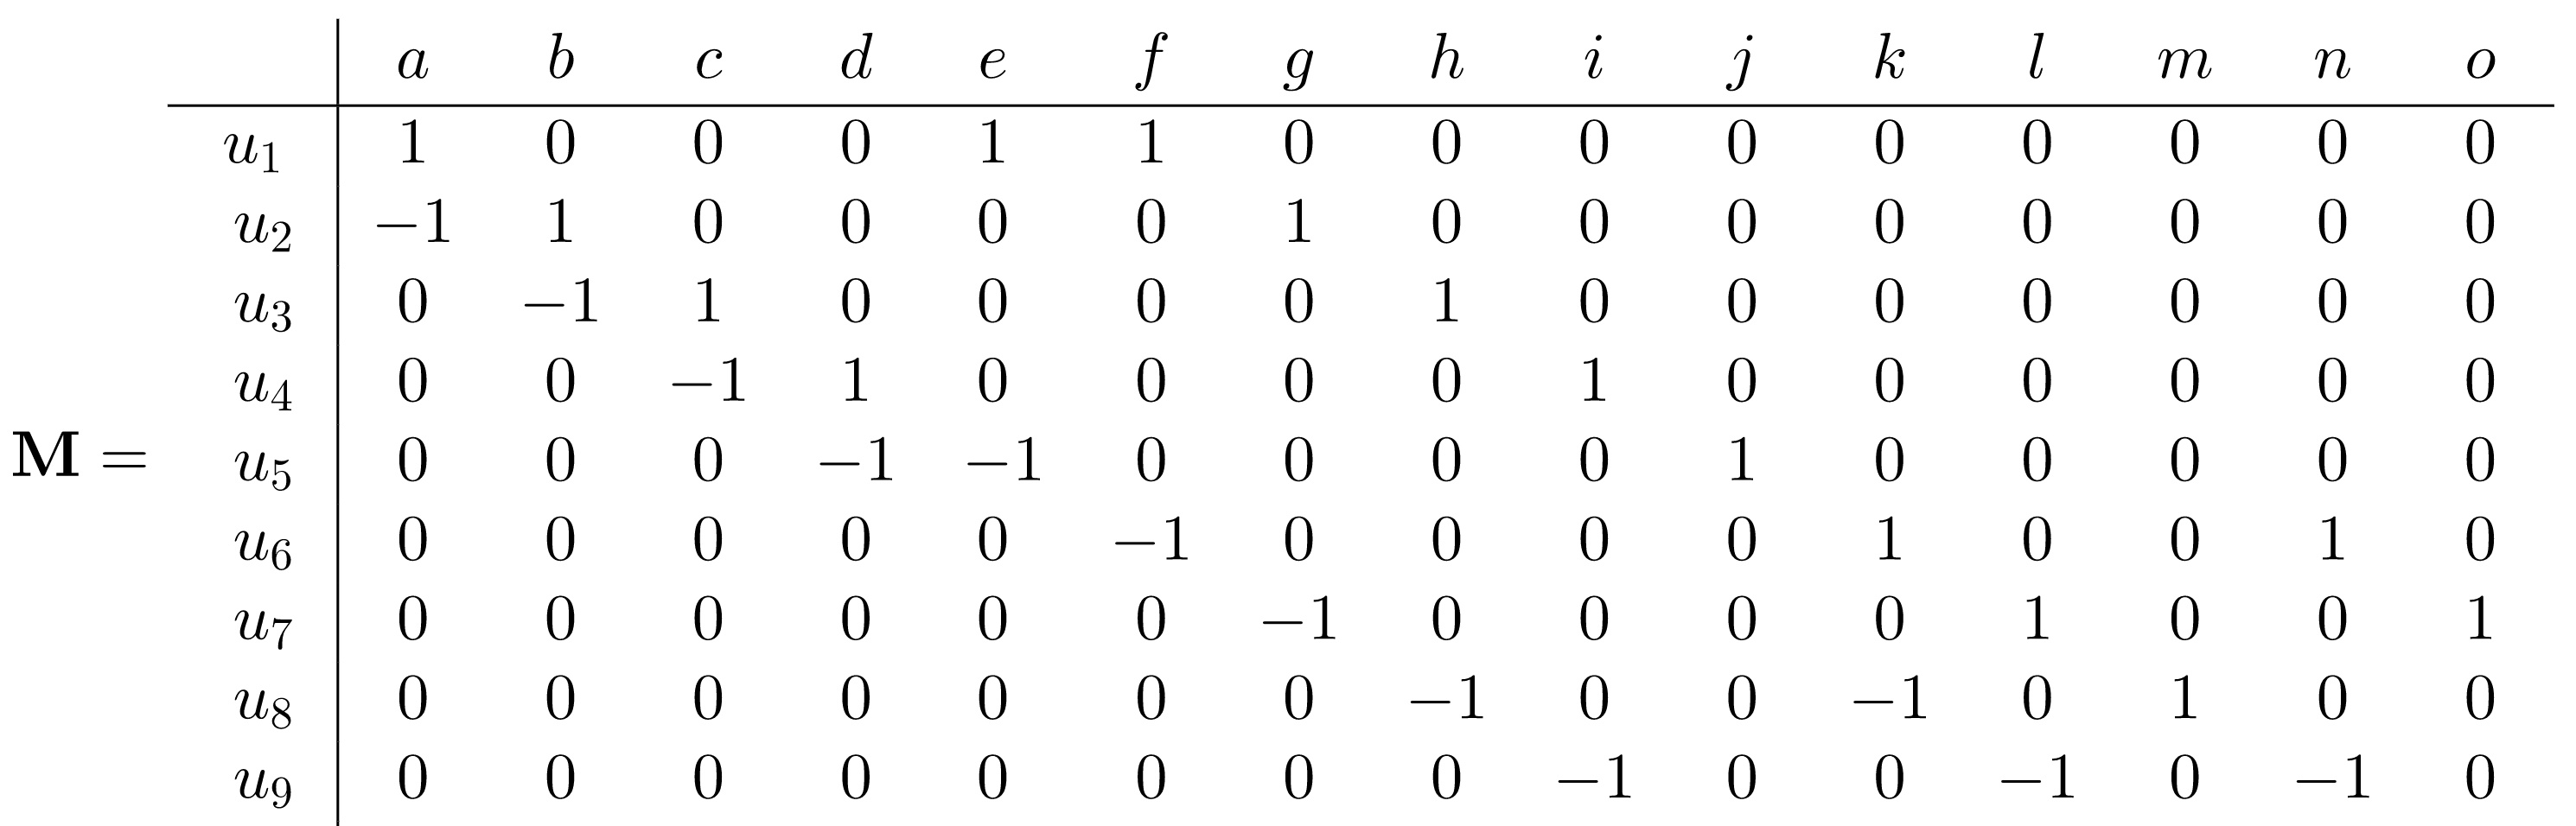
\includegraphics[scale=0.16]{img/imgchapter4/petersendirigido.jpg}
    \caption{}
    \label{fig:petersendirigido}
\end{figure}

Puede probarse que $det(\mathbf{M}\mathbf{M^{t}}) = 2000$. Por tanto, la gráfica de Petersen tiene $2000$ árboles generadores.      

\hfill $\blacklozenge$
\end{ejem}


\section{Redes eléctricas}
A muy grandes rasgos, una \textit{red eléctrica} (en otros contextos también se le conoce como \textit{circuito eléctrico}) es una colección de elementos (o dispositivos) eleéctricos conectados entre sí, tales como resistencias, capacitores, transistores, etc. El comportamiento de estas redes depende de dos factores: las características de los elementos eléctricos involucrados y de qué manera éstos objetos están conectados (o sea, de su \textit{topología}). No profundizaremos en el primer aspecto dado que concierne a sus propiedades \textit{físicas}. Sin embargo, el segundo es de nuestro interés pues es donde la Teoría de Gráficas hace su aparación.

Una red eléctrica se modela con una gráfica, en donde sus aristas corresponden a los dispositivos eléctricos y los nodos que conectan tales elementos son los vértices.

A cada arista $e_{k}$ (o dispositivo) de la red eléctrica se le asocian dos variables en un momento dado $t$: su \textit{voltaje} $v_{k}(t)$ y su corriente $i_{k}(t)$. Puede considerarse al voltaje como aquella variable que representa la  diferencia de potencial de los extremos de la arista; y la corriente es una variable que \textit{fluye} a través de la arista.  Precisamente, para indicar las direcciones de los voltajes y del flujo de las corrientes, es necesario asignarle orientaciones a las aristas de gráfica asociada a la red eléctrica. Por tanto, las redes pueden ser estudiadas a través de las orientaciones de una gráfica. En la figura \ref{fig:dispositivo electrico} mostramos en $(a)$ un elemento de una red eléctrica, y en $(b)$ su arista asociada, junto con su dirección y sus dos variables asociadas. Como una convención, el voltaje $+$ se asume siempre en la cola del arco.

\begin{figure}[H]
    \centering
    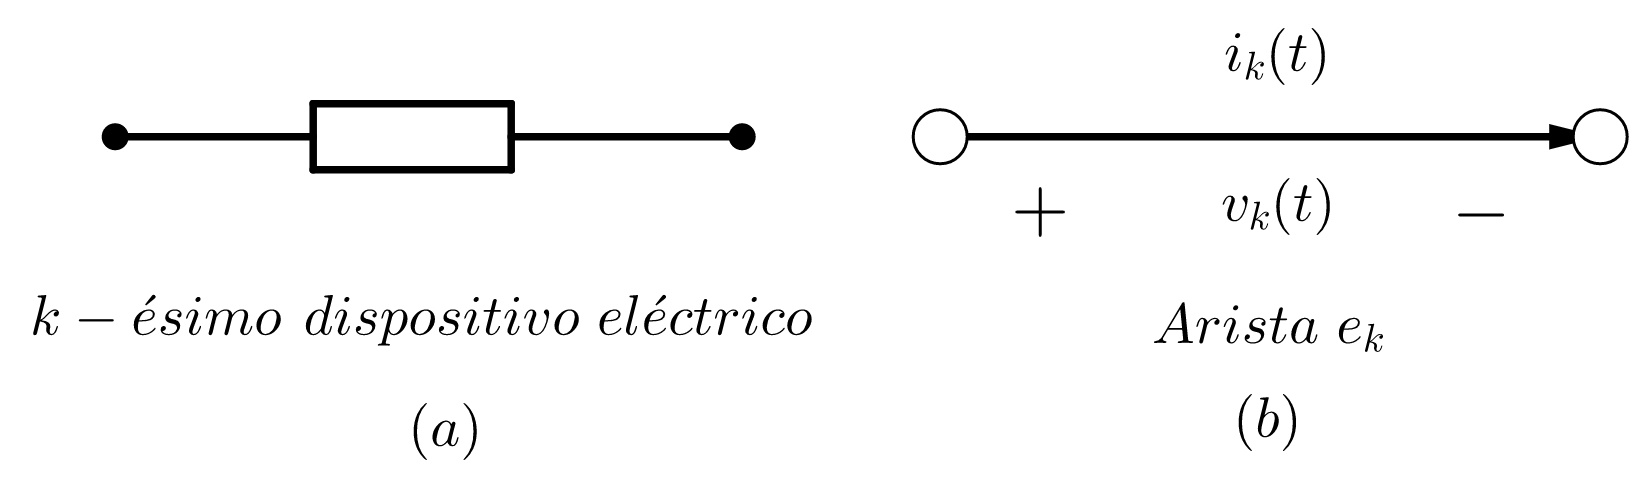
\includegraphics[scale=0.25]{img/imgchapter4/dispositivoelectrico.jpg}
    \caption{}
    \label{fig:dispositivo electrico}
\end{figure}

Supongamos que $G=(V,E)$ representa alguna red eléctrica con $V=\{u_{1}, \ldots, u_{n} \}$ y $E =\{e_{1}, \ldots, e_{m}\}$. Los valores de las corrientes que atraviesan las aristas en un momento $t$ los representamos en un vector columna llamado el \textit{vector de corrientes}:
$$
\mathbf{i}(t): = \begin{bmatrix} 
i_{1}(t) \\
\vdots \\
i_{m}(t)
\end{bmatrix}.
$$

De igual manera, el \textit{vector de voltajes} es el vector columna que representa los voltajes de cada arista en el tiempo $t$:
$$
\mathbf{v}(t): = \begin{bmatrix} 
v_{1}(t) \\
\vdots \\
v_{m}(t)
\end{bmatrix}.
$$

Una de las grandes contribuciones del físico Gustav Kirchhoff (1824 - 1887) fue postular dos leyes que gobiernan el comportamiento de los voltajes y las corrientes de una red eléctrica, en todo tiempo $t$:

\begin{itemize}
    \item \textit{Ley de las corrientes de Kirchhoff:} En cualquier vértice $v$, la suma de las corrientes que entran en ese vértice es igual a la suma de las corrientes que salen. De forma equivalente, la suma de todas las corrientes que pasan por el vértice es igual a cero:$$ \sum_{a \in \partial(v)} i_{a}(t) = 0$$
    \item \textit{Ley de los voltajes de Kirchhoff:} La suma de todas las voltajes en un ciclo $C$ de la red eléctrica es igual a cero: $$\sum_{a \in E(C)} v_{a}(t) = 0$$
\end{itemize}

En la primera ley consideramos las direcciones de las aristas (y los signos $+$ y $-$ de los voltajes); y en la segunda se considera de antemano una orientación arbitraria de los ciclos. Por ejemplo, consideremos la red eléctrica de la figura \ref{fig:redelectrica}.

\begin{figure}[H]
    \centering
    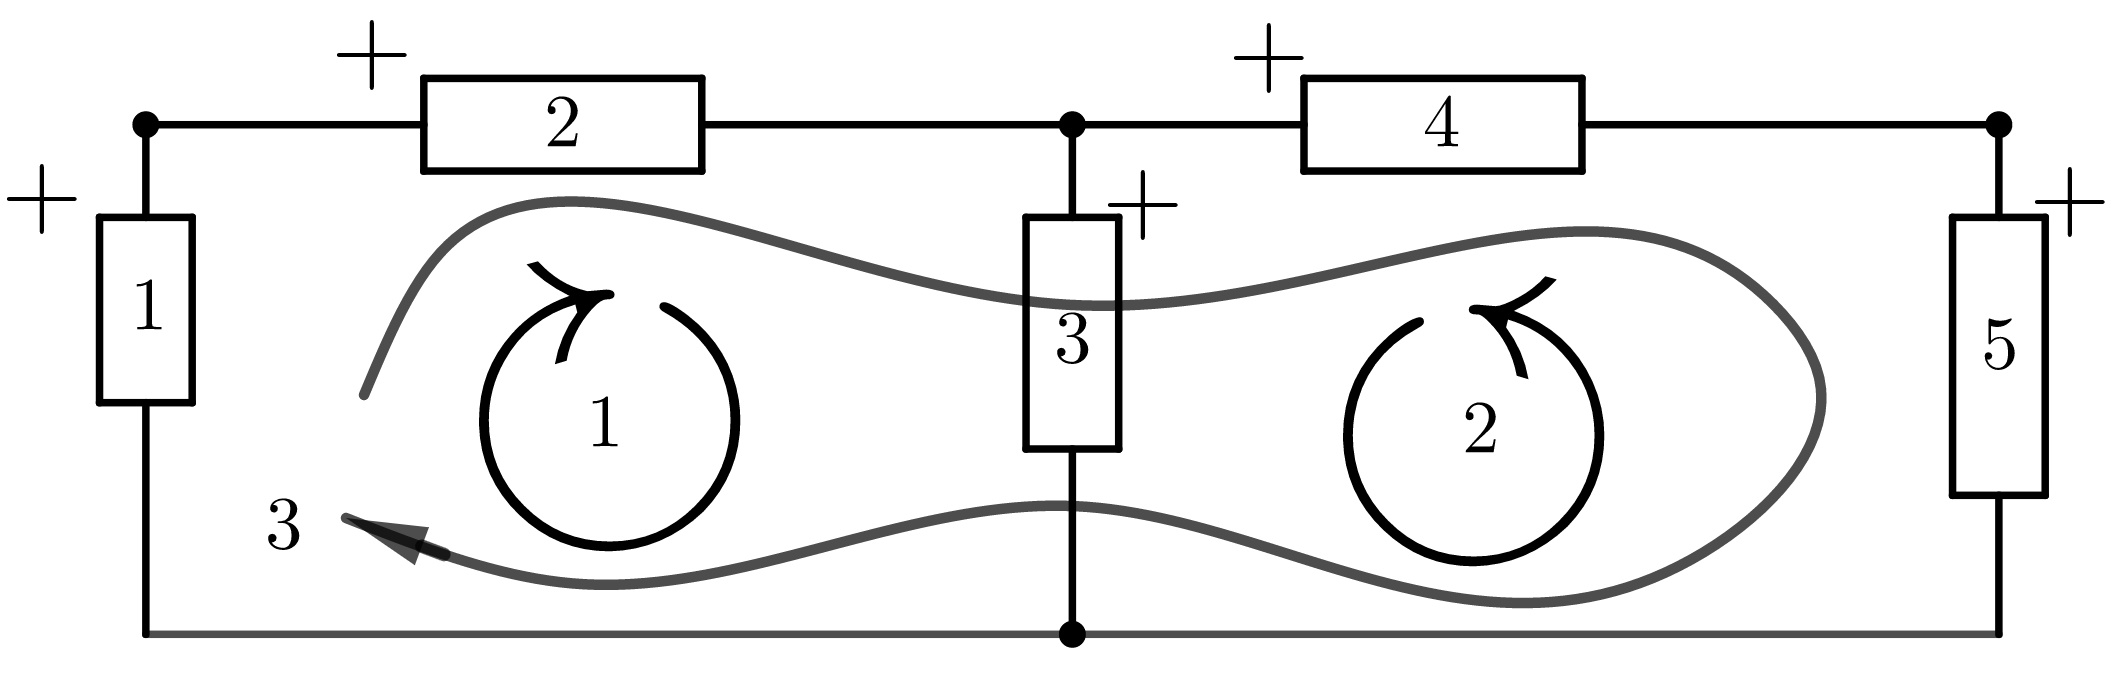
\includegraphics[scale=0.25]{img/imgchapter4/redelectrica.jpg}
    \caption{}
    \label{fig:redelectrica}
\end{figure}

Los signos $+$ nos dicen en qué dirección van los voltajes y las corrientes. También indicamos la orientación de los ciclos de la red. En la figura \ref{fig:redelectricagraficaasociada} colocamos la digráfica $D$ asociada, mostrando también las orientaciones de los arcos y los ciclos.

\begin{figure}[H]
    \centering
    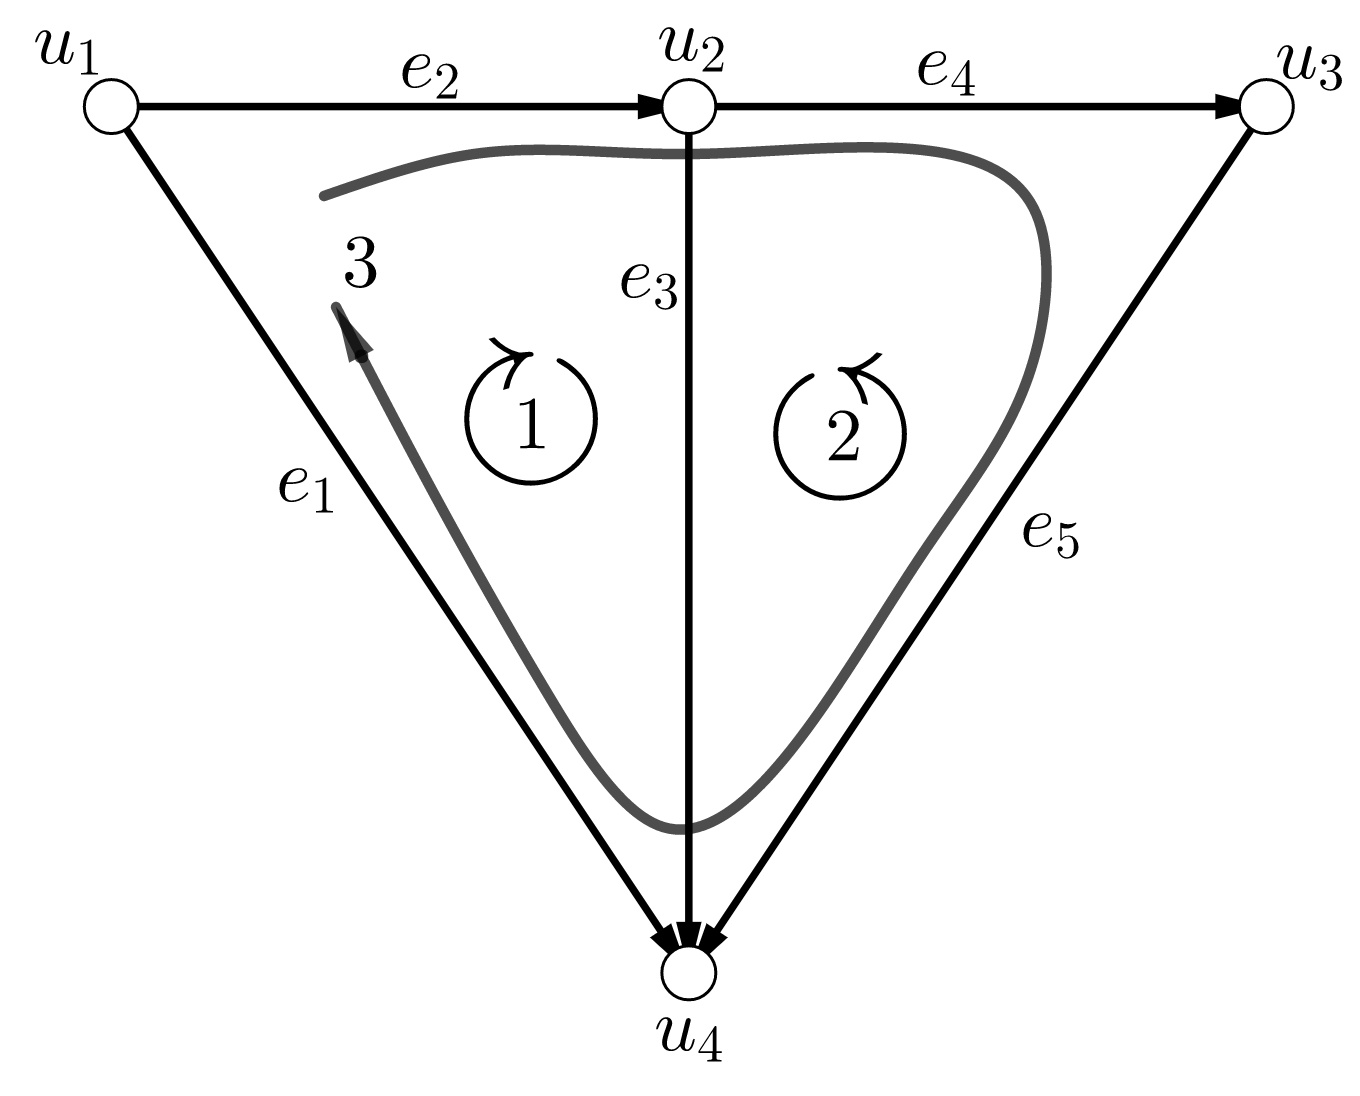
\includegraphics[scale=0.2]{img/imgchapter4/redelectricagraficaasociada.jpg}
    \caption{}
    \label{fig:redelectricagraficaasociada}
\end{figure}

Así, según las leyes de Kirchhoff, tenemos las siguientes ecuaciones:

\begin{itemize}
    \item \textit{Ecuaciones de las corrientes:}
    \begin{align*}
    \textnormal{Vértice }u_{1} &:&  &i_{1}(t)&  &+& &i_{2}(t)& & &   & &      & & & &        && && &=&0  \\  
    \textnormal{Vértice }u_{2} &:&    &&        &-& &i_{2}(t)& &+& &i_{3}(t)& &+& &i_{4}(t)& && && &=& 0 \\
    \textnormal{Vértice }u_{3} &:&    &&        & & & & & & & &               &-& &i_{4}(t)& &+& &i_{5}(t)& &=& 0 \\
    \textnormal{Vértice }u_{4} &:&  &-i_{1}(t)& & & & & &-& &i_{3}(t)& & & & & &-& &i_{5}(t)& &=& 0
    \end{align*}
    
    \item \textit{Ecuaciones de los voltajes:}
        \begin{align*}
   \textnormal{Ciclo }1 &:&  &-v_{1}(t)&  &+& &v_{2}(t)& &+&   &v_{3}(t) &      & & & &        && && &=&0  \\  
   \textnormal{Ciclo }2 &:&    &&        & & & & & & &v_{3}(t)& &-& &v_{4}(t)& &-& &v_{5}(t)& &=& 0 \\
   \textnormal{Ciclo }3 &:&  &-v_{1}(t)&   &+& &v_{2}(t)& & &  & & &+& &v_{4}(t)& &+& &v_{5}(t)& &=& 0 \\
    \end{align*}
\end{itemize}

En notación matricial, las ecuaciones de las corrientes y voltajes se expresan como:

\begin{align*}
\begin{bmatrix}
1 & 1 & 0 & 0 & 0\\ 
0 &-1  & 1 & 1 & 0\\ 
0 & 0 & 0 & -1 & 1\\ 
-1 & 0 & -1 & 0 & -1
\end{bmatrix} \begin{bmatrix}
i_{1}(t)\\ 
i_{2}(t)\\ 
i_{3}(t)\\ 
i_{4}(t)\\ 
i_{5}(t)
\end{bmatrix}&=\begin{bmatrix}
0\\ 
0\\ 
0\\ 
0
\end{bmatrix} \\
\begin{bmatrix}
-1 & 1 & 1 & 0 & 0\\ 
0 &0  & 1 & -1 & -1\\ 
-1 & 1 & 0 & 1 & 1
\end{bmatrix} \begin{bmatrix}
v_{1}(t)\\ 
v_{2}(t)\\ 
v_{3}(t)\\ 
v_{4}(t)\\ 
v_{5}(t)
\end{bmatrix}&=\begin{bmatrix}
0\\ 
0\\ 
0
\end{bmatrix}    
\end{align*}

Si observamos atentamente, podemos darnos cuenta que las matrices asociadas a las corrientes y a los voltajes son, respectivamente, las matrices de incidencia y de ciclos de la digráfica que representa a la red eléctrica. Entonces el vector de corrientes está en el kernel de la matriz de incidencia, i.e., es una circulación del espacio $\mathcal{C}(D)$; y el vector de voltajes está en el kernel de la matriz de ciclos, o sea, es una tensión del espacio $\mathcal{B}(D)$. Por estas razones, los espacios $\mathcal{B}(D)$ y $\mathcal{C}(D)$ recibieron sus nombres.

Este fenómeno no es exclusivo del ejemplo previo, es algo que sucede en general, cualquiera que sea la cantidad de vértices o de aristas.

Gracias a la herramientas desarrolladas en esta tesis, las leyes de Kirchhoff se reformulan como sigue:

\begin{itemize}
    \item \textit{Ley de las corrientes de Kirchhoff:} La corrienes de una red eléctrica forman un circulación de la digráfica asociada, es decir: $$
    \mathbf{M}\cdot\mathbf{i}(t) = \mathbf{0}.$$
    
    \item \textit{Ley de los voltajes de Kirchhoff:} Los voltajes de una red eléctrica forman una tensión de la digráfica asociada, o sea: $$
    \mathbf{B}\cdot\mathbf{v}(t) = \mathbf{0}.$$
\end{itemize}


Parte del trabajo de Kirchhoff fue determinar qué ecuaciones de las corrientes y los voltajes eran linealmente independientes. Ahora podemos afirmar que, necesariamente, hay $n-1$ ecuaciones de las corrientes linealmente independientes; y $m -n +1$ ecuaciones de los voltajes linealmente independientes. Aún más, estas ecuaciones se obtienen a partir de un árbol generador de la red y considerando las matrices $\widehat{\mathbf{M}}$ y $\mathbf{B}_{f}$. 

Hay una cantidad considerable de literatura que trata estos temas. El lector interesado puede consultar \cite{Deo,Seshu,Slepian,Chen}.

\section{Gráficas planas}

Los conjuntos de corte y los ciclos (y las gráficas pares, en general) parecen estar íntimamente ligados, como ha quedado demostrado en todo este trabajo. Pareciera, incluso, que tiene un comportamiento dual. Comentaremos esta noción de dualidad desde un punto de vista más formal.

No será nuestro objetivo hacer un estudio de las gráficas planas\footnote{El libro \cite{Bondy} es una excelente referencia al respecto. Sin embargo, también puede hallarse información en \cite{Chen,Deo,Diestel,Seshu,Gross}}. No obstante, es necesario hacer algunas observaciones al respecto. Como el lector sabrá, en términos muy generales, decimos que una gráfica es \textit{plana} si es posible dibujarla en un plano de tal manera que sus aristas sólo se corten en sus extremos (y no en otros puntos del plano).

Ejemplos de gráficas no planas son $K_{5}$ y $K_{3,3}$, ni lo son, tampoco, ninguna de sus subdivisiones. Una subdivisión de una gráfica $G$ es una gráfica que resulta de subdividir aristas de $G$. De hecho,  Kazimierz Kuratowski (1896 - 1980) probó lo siguiente:

\begin{teo}[\textbf{\textit{Teorema de Kuratowski}}]
Una gráfica es plana si y sólo si no contiene subdivisiones de $K_{5}$ o de $K_{3,3}$.
\end{teo}

Cada gráfica plana \textit{particiona} al plano en un número finito $f$ de regiones conexas por trayectorias. Tales regiones son llamadas las \textit{caras de la gráfica}. Una de estas caras siempre será no acotada, la cual se llama \textit{cara exterior}. En la figura \ref{fig:plana} se muestra una gráfica plana junto con sus caras.

\begin{figure}[h]
    \centering
    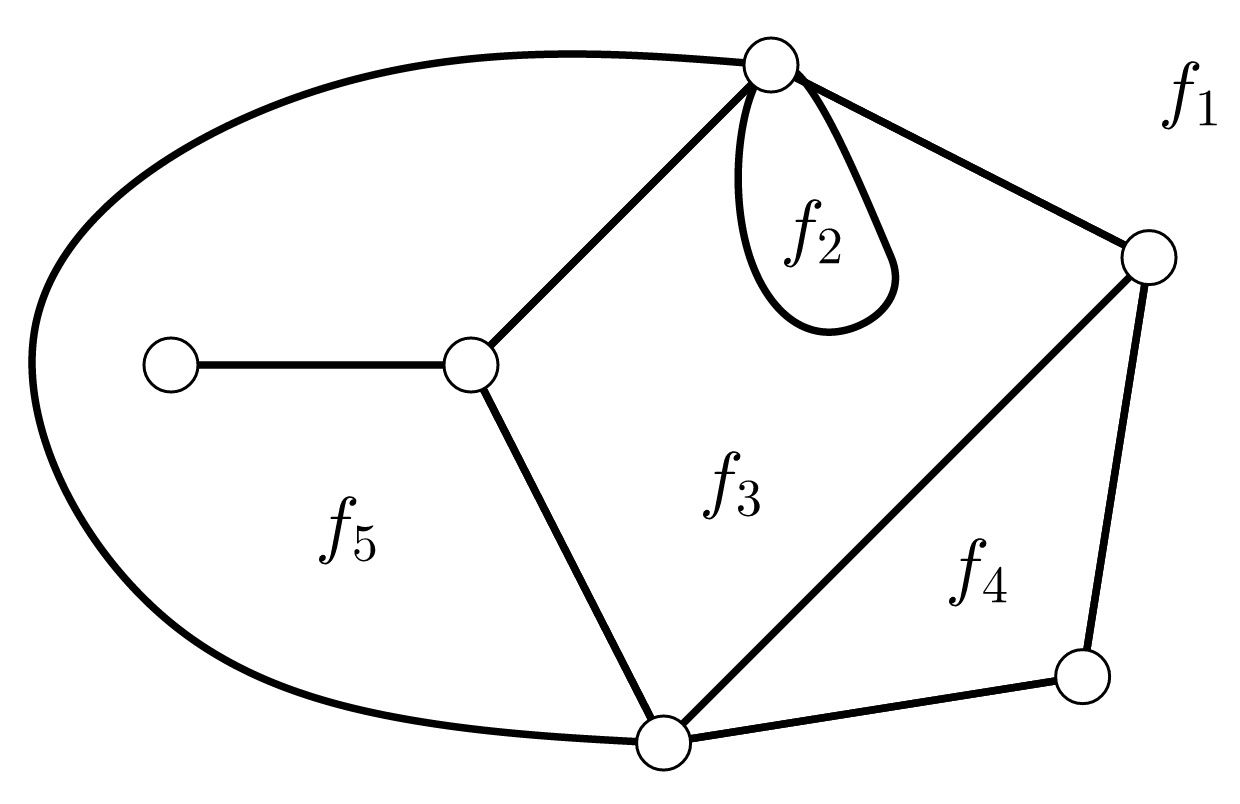
\includegraphics[scale=0.2]{img/imgchapter4/graficaplana.jpg}
    \caption{}
    \label{fig:plana}
\end{figure}

Si $G$ es plana, podemos construir otra gráfica $G^{*}$ donde sus vértices corresponden a las caras de $G$ y éstos son adyacentes si sus caras respectivas son separadas por una arista. A cada arista $e$ de $G$, le corresponde una arista $e*$ en $G^{*}$. Véase la figura \ref{fig:dual}, en donde dibujamos el dual de la gráfica de la figura \ref{fig:plana}. Se sabe que $G^{*}$ es plana; y que si $G$ es conexa, $G^{*}$ también es conexa.
\begin{figure}[H]
    \centering
    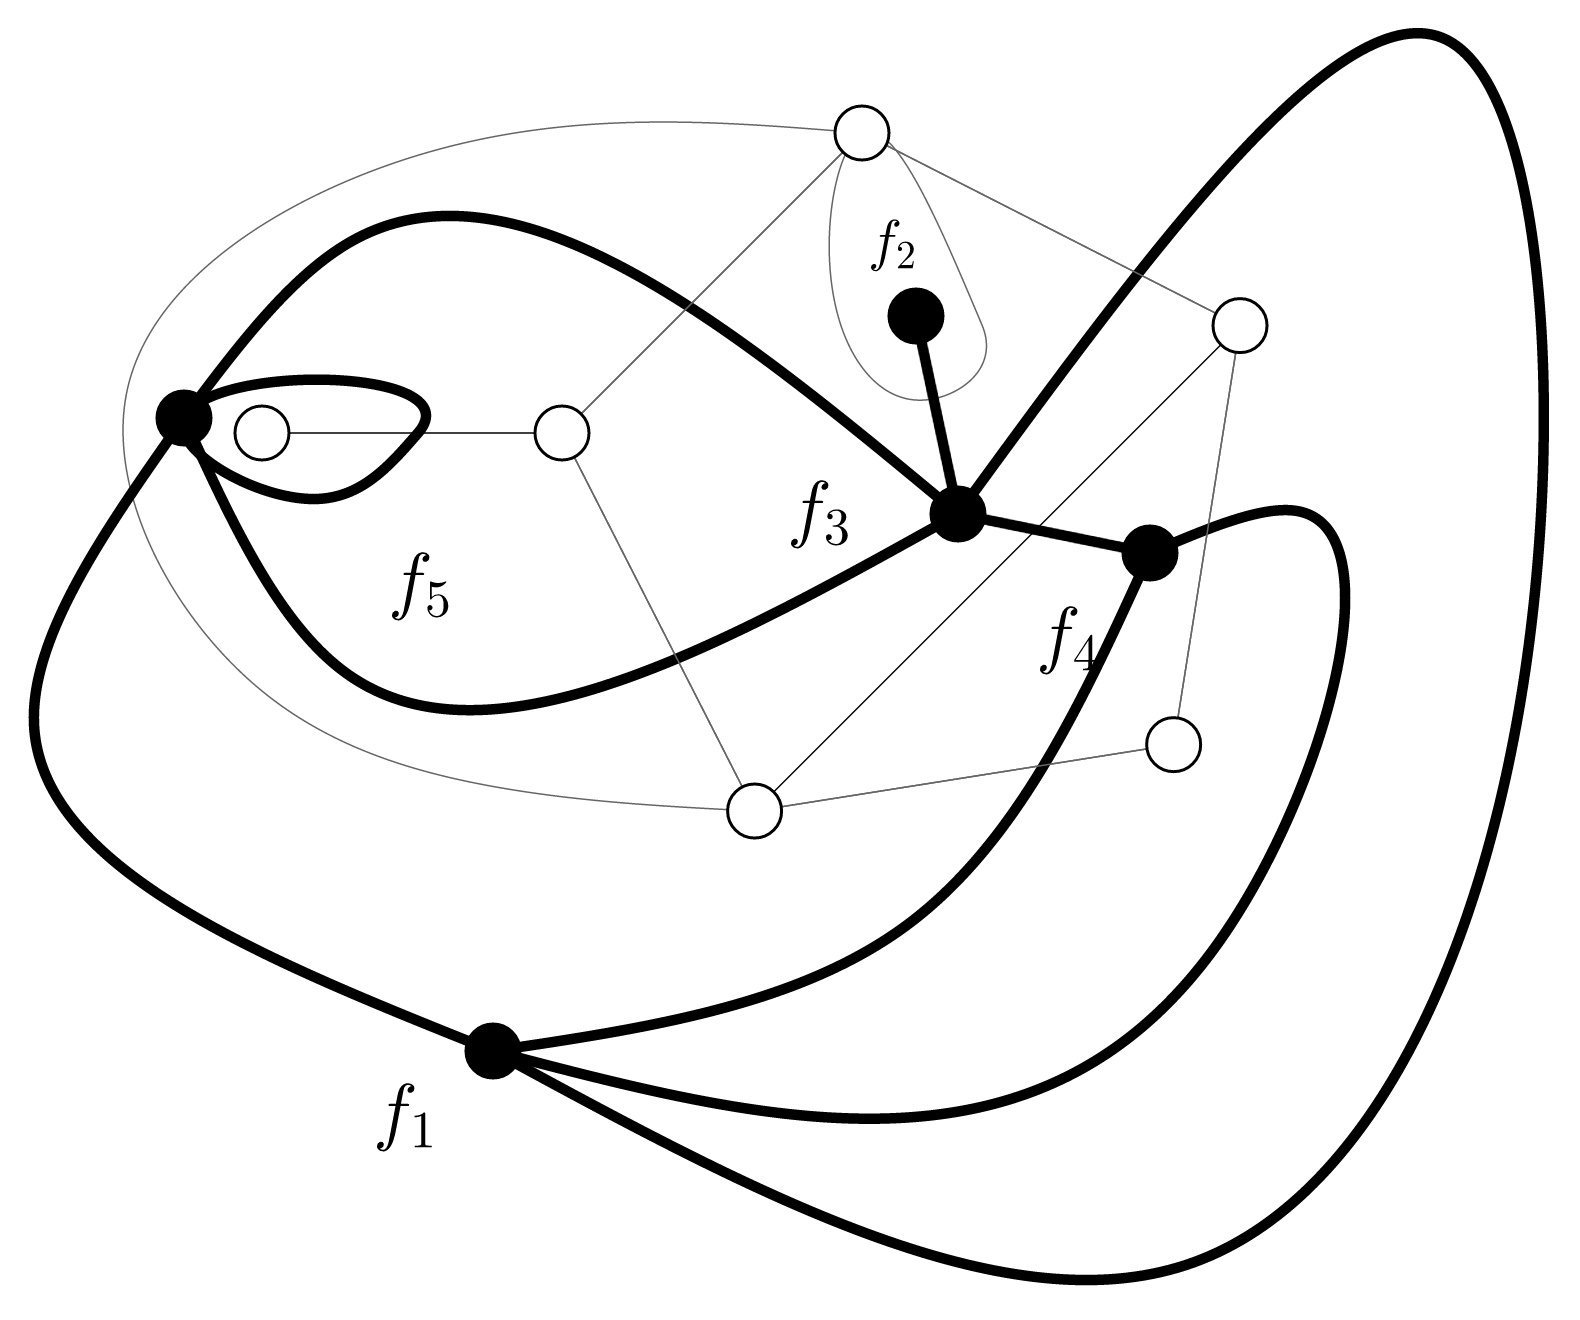
\includegraphics[scale=0.2]{img/imgchapter4/dual.jpg}
    \caption{}
    \label{fig:dual}
\end{figure}

Si $S\subseteq E(G)$, escribimos $S^{*} = \{e^{*} | e\in S\} \subseteq E(G^{*})$. Las propiedades más relevante que nos conciernen las enunciamos como un teorema y un corolario:

\begin{teo}
Sea $G$ una gráfica plana y conexa y consideremos su dual $G^{*}$. Se cumple lo siguiente: 
\begin{itemize}
    \item Si $C$ es un ciclo de $G$, entonces $C^{*}$ es un corte minimal en $G^{*}$.
    \item Si $B$ es un corte minimal en $G$, entonces $B^{*}$ es un ciclo de $G^{*}$.
\end{itemize}
\end{teo}

\begin{cor}
Para toda gráfica plana $G$, el espacio de ciclos de $G$, $\mathcal{C}(G)$, es isomorfo al espacio de cortes de $G^{*}$, $\mathcal{B}(G^{*})$.
\end{cor}

El teorema de Kuratowski caracteriza las gráficas planas de una manera muy \textit{geométrica}. Durante algún tiempo se buscó una caracterización menos \textit{topológica} y más \textit{combinatoria} (o más bien, \textit{algebraica}). Quien logró tal hazaña fue el matemático Hassler Whitney (1907-1989) en los años $30$ del siglo XX, en una serie de famosos artículos.

Whitney estudió las relaciones que hay entre una gráfica y su \textit{dual geométrico} y propuso una noción de dualidad más abstracta. El objetivo entonces era probar que dos gráficas duales geométricamente, también lo eran en el sentido de Whitney, y viceversa.

Supongamos que tenemos dos gráficas $G_{1}$ y $G_{2}$, y una función biyectiva $\theta \colon E(G_{1}) \rightarrow E(G_{2})$. Entonces podemos construir otra función biyectiva $\boldsymbol{\theta} \colon \mathcal{E}(G_{1}) \rightarrow \mathcal{E}(G_{2})$ que manda una subgráfica generadora de $G_{1}$ en la correspondiente subgráfica generadora de $G_{2}$, vía $\theta$; es decir, que para toda $H \in \mathcal{E}(G_{1})$, $$\boldsymbol{\theta}(H):= G_{2}[\theta(E(H)] \in \mathcal{E}(G_{2})$$.

Decimos que dos gráficas $G_{1}$ y $G_{2}$ son \textit{duales en el sentido de Whitney} (o también que son \textit{duales algebraicamente}) si existe una función $\theta \colon E(G_{1}) \rightarrow E(G_{2})$ tal que, para toda $H\in \mathcal{E}(G_{1})$, se cumple:
$$\rho(G_{2} \setminus \boldsymbol{\theta}(H)) = \rho(G_{2}) - \mu(H).$$

Equivalentemente, $G_{1}$ y $G_{2}$ son \textit{duales en el sentido de Whitney} si existe una función $\theta \colon E(G_{1}) \rightarrow E(G_{2})$ tal que $C \in \mathcal{E}(G_{1})$ es un ciclo de $G_{1}$ si y sólo si $\boldsymbol{\theta}(C)$ es un corte minimal de $G_{2}$.

Whitney logró demostrar que \textit{ni $K_{5}$ ni  $K_{3,3}$ tiene duales algebraicos}. Aún más, probó que \textit{toda gráfica es plana si y sólo si tiene un dual algebraico}. Finalmente, \textit{que toda gráfica tiene un dual algebraico si y sólo si no contiene subdivisiones de $K_{5}$ ni de $K_{3,3}$}; logrando así una caracterización algebraica de las gráficas planas.

\section{Optimización Combinatoria}
La Optimización Combinatoria es una rama de las Matemáticas que, para resolver los problemas que se plantea, se vale de otras ramas y técnicas de combinatoria. Su uso de la Teoría de Gráficas y el Álgebra Lineal es frecuente.

En esta sección mencionaremos brevemente cómo la teoría presentada en este trabajo ha sido, de una u otra manera, útil para Optimización Combinatoria. A continuación, describiremos algunos de los problemas más famosos que se han estudiado.

Dada una gráfica, un \textit{apareamiento} es un subconjunto de aristas que no tienen vértices extremos en común. El apareamiento es \textit{perfecto} si todo vértice de la gráfica es extremo de alguna arista del apareamiento.

El estudio de los apareamientos en gráficas ha sido productivo. Por ejemplo, los problema de encontrar un apareamiento de cardinalidad máxima y el de hallar un aparemiento de peso máximo (otorgándole pesos a las aristas) pueden ser modelados usando las herramientas que trabajamos en los capítulos anteriores. 

Otro es el \textit{problema de asignación} que consiste en encontrar un apareamiento perfecto de peso mínimo. De forma similar, hallar un árbol generador de peso máximo o peso mínimo son problemas clásicos

El lector encontrará en \cite{Korte} una excelente fuente para profundizar en estos temas.

Las redes de comunicación y de transporte han generado también diversas cuestiones que se han contestado gracias a la Optimización Combinatoria. El estudio de las redes involucra un concepto similar (y de cierto modo, equivalente) a las circulaciones en digráficas.

\subsection{Flujo en redes}
Una \textit{red} es una cuádrupla $N:=(D,c,s,t)$ en donde $D$ es una digráfica junto con dos vértices distinguidos: una fuente $s$ y un pozo $t$; y una función no negativa $c\colon A(D) \rightarrow \mathbb{R}$. Los demás vértices de la red son llamados \textit{vértices intermedios} e $I$ denota el conjunto de éstos. La función $c$ es conocida como la \textit{función de capacidad} de la red $N$, y cada valor $c(a)$ es la \textit{capacidad} del arco $a$. A veces a $D$ se le llama la \textit{digráfica subyacente} de la red $N$.

Un \textit{flujo} en $N$ es una función $f\colon A(D) \rightarrow \mathbb{R}$ que satisface la condición de conservación en sus vértices internos, i.e., para todo $v \in I$,$$ F^{+}(v) - F^{-}(v) = 0.$$

Se dice que un flujo es \textit{factible} si satisface la \textit{restricción de capacidad}: $$0 \leq f(a) \leq c(a), \textnormal{ para todo } a \in A(D).$$

un $s-t$ \textit{corte} en la red $N$ es un excorte $\partial^{+}(X)$ de su digráfica subyacente, de tal forma que $s \in X$ y $t\in \overline{X}$. La capacidad de un $s-t$ corte es la suma de las capacidades de sus arcos, es decir:$$cap(\partial^{+}(X)):=\sum_{a \in \partial^{+}(X)}c(a) = C^{+}(X)$$.

Por otro lado, dado $X\subseteq V(D)$, el \textit{flujo que sale} de $X$ es el número $F^{+}(X)- F^{-}(X)$ y el \textit{flujo que entra} en $X$ es $F^{-}(X)- F^{+}(X)$. Puede probarse que la cantidad  $F^{+}(X)- F^{-}(X)$ es constante, dado cualquier subconjunto $X$ que cumpla que $s \in X$ y $t\in \overline{X}$. Este número es el \textit{valor del flujo $f$} y se escribe $val(f)$.

Un $s -t$ corte es un \textit{corte mínimo} si no hay otro $s-t$ corte en $N$ de menor capacidad; y un flujo $f$ es de \textit{flujo máximo} si no hay otro flujo de mayor valor. 

Los $s -t$ cortes y los flujos están íntimamente relacionados. Por ejemplo, dado cualquier $s-t$ corte $K$ y cualquier flujo $f$, se sabe que $val(f) \leq cap(K)$. Aún más, si $val(f) = cap(K)$, necesariamente $f$ es un flujo máximo y $K$ un corte  mínimo.

Uno de los problemas más famosos de la Optimización Combinatoria es de encontrar un flujo máximo en una red dada. El algortimo más famoso para resolverlo es el de Ford y Fulkerson, publicado en los años 50 del siglo XX. El teorema que sigue es un resultado central que caracteriza los flujos máximos en redes y los cortes de capacidad mínima.

\begin{teo}[\textbf{\textit{El teorema Máximo Flujo Mínimo Corte}}]
En toda red, el valor de un flujo máximo es igual a la capacidad de un corte mínimo
\end{teo}

El teorema anterior es una generalización de otro resultado ampliamente conocido en la Teoría de Gráficas: dando el valor de $1$ a las capacidades de cada arco de una red, se deduce el Teorema de Menger.

\begin{teo}[\textbf{\textit{Teorema de Menger}}]
En cualquier digráfica con dos vértices distinguidos $s$ y $t$, el número máximo de $(s,t)-$trayectorias ajenas por aristas (dos a dos) es igual al mínimo número de arcos en un $s-t$ corte.
\end{teo}

Finalmente, asignando pesos y costos a los arcos e imponiendo otras restricciones, los famosos problemas de Programación Lineal tales como el de \textit{la ruta más corta}, \textit{asignación óptima}, \textit{el problema de transporte} y el de \textit{transbordo}, han sido modelados en términos de flujos en redes, encontrándose que son equivalentes. Los libros \cite{FordFulkerosns, Chen, Chen2, Bondy, Korte} tratan con más detalle el estudio de los flujos en redes.

\subsection{Matroides}
En el capítulo 3 de esta tesis pudimos darnos cuenta de cómo se relacionan las matrices de incidencia con los espacios vectoriales asociados a las gráficas. Nos dimos cuenta también cómo las bases del espacio de columnas de dicha matriz corresponden a los árboles (bosques maximales) generadores de la gráfica; así como los ciclos corresponden a los conjuntos de columnas linealmente dependientes.

Inspirado en estos fenónemos, Whitney dio un paso más allá en su artículo \cite{Whitney1935} de 1935 generalizando a la vez los espacios vectoriales y las gráficas en una nueva estructura llamada \textit{matroide}. Así, el estudio de los matroides es el estudio de una teoría abstracta de la dependencia lineal\footnote{Un buen libro para estudiar la Teoría de Matroides es \cite{Oxley}}.

Un matroide $M$ es un par ordenado $(E,\mathcal{I})$ que consiste de un conjunto finito $E$ y una colección $\mathcal{I}$ de subconjuntos de $E$ con las siguientes propiedades:

\begin{itemize}
    \item $\emptyset \in \mathcal{I}$
    \item Si $I\in \mathcal{I}$ e $I' \subseteq I$, entonces $I'\in \mathcal{I}$.
    \item Si $I_{1}$ e $I_{2}$ pertenecen a $\mathcal{I}$ y $|I_{1}|<|I_{2}|$, entonces existe un elemento $e \in I_{2} \setminus I_{1}$ tal que $I_{1} \cup \{e\} \in \mathcal{I}.$
\end{itemize}

Los elementos de $\mathcal{I}$ son conocidos como \textit{conjuntos independientes} del matroide $M$. Los \textit{conjuntos dependedientes de} $M$ son los subconjuntos de $E$ que no pertencen a $\mathcal{I}$. los \textit{circuitos} son los conjuntos dependientes minimales de $M$. Los conjuntos independientes maximales reciben el nombre de \textit{bases de} $M$. 

De hecho, los matroides pueden ser definidos de manera equivalente por medio de sus bases. El siguiente párrafo expresa estas ideas.

Un matroide es un par ordenado $(E, \mathcal{B})$ que consiste de un conjunto finito $E$ y una colección $\mathcal{B}$ de subconjuntos de $E$ llamados \textit{bases}, que satisfacen dos condiciones:
\begin{itemize}
    \item $\mathcal{B} \neq \emptyset$
    \item \textit{Propiedad de intercambio.} Si $B_{1}$ y $B_{2}$ son dos bases y $e \in B_{1}\setminus B_{2}$, entonces existe $f \in B_{2}\setminus B_{1}$ tal que $(B_{1} \setminus \{e\})\cup \{f\} \in \mathcal{B}$.
\end{itemize}

Entonces los conjuntos independientes de un matroide son subconjuntos de sus bases. Por ejemplo, una matriz $\mathbf{M}$ con entradas en un campo $\mathbb{F}$ da pie al \textit{matroide lineal} $(E, \mathcal{B})$ en donde $E$ es el conjunto de columnas de $\mathbf{M}$ y $\mathcal{B}$ el conjunto de todas las bases del espacio de columnas de $\mathbf{M}$.

El \textit{matroide gráfico} $M(G):= (E, \mathcal{B})$ asociado a una gráfica $G$ es aquel donde $E$ es el conjunto de aristas de $G$ y $\mathcal{B}$ los conjuntos de aristas correspondientes a los bosques generadores maximales de $G$. En ese caso, los conjuntos independientes son las subgráficas acíclicas y los circuitos son los ciclos de $G$.

El \textit{dual} de un matroide $M$ es el matroide $M^{*} = (E,\mathcal{B}^{*})$ donde $\mathcal{B}^{*}:=\{E\setminus B | B \in \mathcal{B}\}$. En cuanto al matroide gráfico $M(G)$, las bases de su dual $M^{*}(G)$ son los complementos de los bosques generadores maximales y sus circuitos son los conjuntos de corte minimales. $M^{*}(G)$ es conocido como el \textit{matroide co-gráfico}.

Al principio de esta sección mencionamos algunos problemas de maximización y de minización. Resulta que, gracias a su estructura, incluso éstos pueden ser generalizados con matroides.

El \textit{Problema de Maximización} en matroides puede ser formulado como sigue: dado un matroide $M=(E,\mathcal{I})$ con pesos en los elementos de $E$, es decir, una función no negativa $c \colon E \rightarrow \mathbb{R}$, hallar un conjunto independiente $X$ de peso máximo, o sea, $X\in \mathcal{I}$ tal que $C(X) = \sum_{e \in X}c(e)$ es máximo.

El \textit{Problema de Minimización} se establece de forma análoga: dado un matroide $M=(E,\mathcal{B})$ con pesos en los elementos de $E$, encontrar una base de peso mínimo.

Otros problemas conocidos son aquellos que involucran la intersección de matroides. Si $(E,\mathcal{I}_{1})$ y $(E,\mathcal{I}_{2})$ son dos matroides sobre el mismo conjunto $E$, su \textit{intersección} es el sistema de conjuntos $(E,\mathcal{I}_{1} \cap \mathcal{I}_{2})$. Aunque, en general, tal intersección no es un matroide, es de interés hallar el conjunto $X \in \mathcal{I}_{1} \cap \mathcal{I}_{2} $ de cardinalidad máxima; más aún, si los matroides tienen pesos, encontrar $X \in \mathcal{I}_{1} \cap \mathcal{I}_{2}$ de peso $c(X)$ máximo. El problema de encontrar un apareamiento de cardinalidad máxima en una gráfica bipartita puede modelarse en términos de una intersección de matroides.

\section{Conclusión}
Podemos darnos cuenta que la Teoría de Matroides es útil por su poder de generalización y sus apliaciones. Es por esto que los matemáticos se han esforzado en estudiar y desarrollar teoría y algoritmos para matroides. A manera de conclusión, los matroides son, de cierto modo, una conclusión de los temas revisados en la presente tesis, y un comienzo para nuevas áreas cuyas influencias siguen repercutiendo en las Matemáticas hasta nuestros días.